%!TEX root = ../thesis.tex
\chapter{Context generalisation}

\label{ch:Context}

Structures such as smap and if, which alter control flow and thus have implications on the working of the \yauhau{} base transformation do not just occur independently in code.
As was mentioned in Chapter \ref{ch:smap-transformation} these structures can be nested.
However even though the smap transformation correctly handles smaps nested in smaps to arbitrary depth we may also have interleaved nesting of smap and if, see Figure~\ref{fig:nested-context-example} and \ref{fig:visual-context-nesting-example-exploded}.

\begin{figure}
\begingroup
\definecolor{green(html/cssgreen)}{rgb}{0.0, 0.5, 0.0}
\catcode`\@=\active
\def@#1@{\textcolor{green(html/cssgreen)}{#1}}
\begin{minted}[escapeinside=||]{Clojure}
(|@defalgo@| algo1 [param]
  (smap
    (|@algo@| [val]
      (if (is-iterable? val)
        (smap (|@algo@| [item] (compute-something (fetch item)))
          val)
        (some-operation val))))
\end{minted}
\endgroup
\caption{Nested context example}
\label{fig:nested-context-example}
\end{figure}

\begin{figure}
    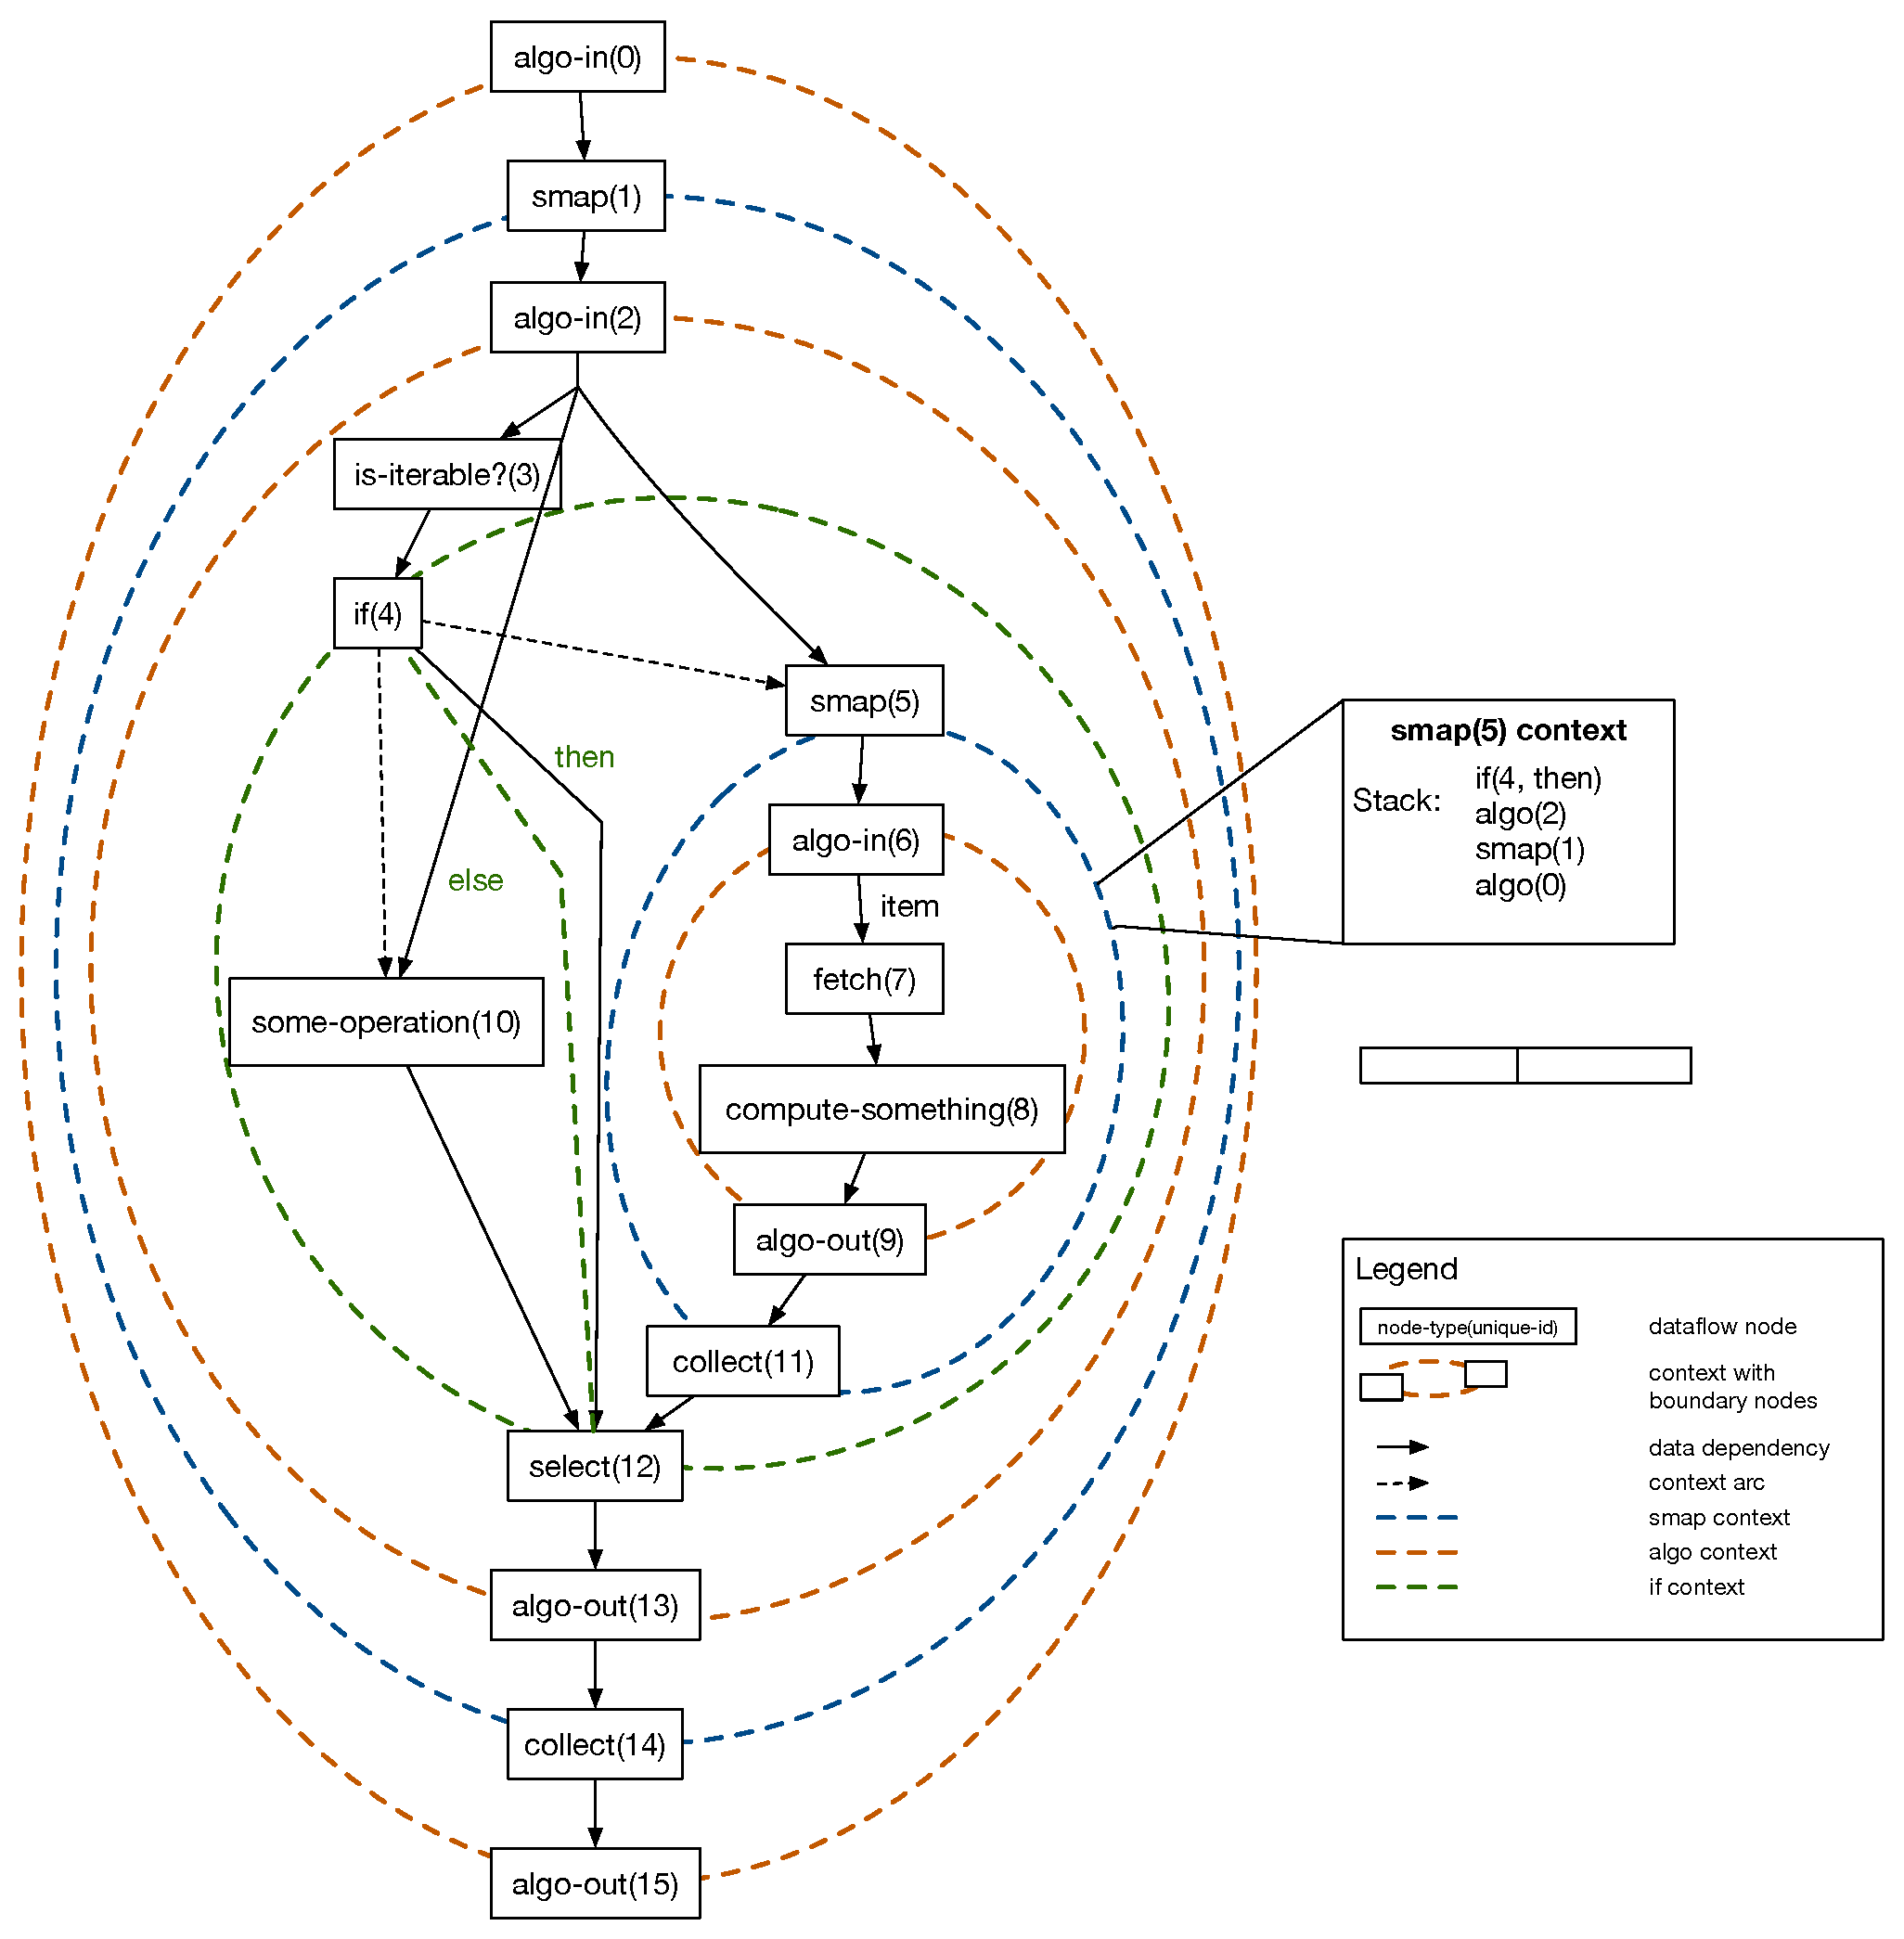
\includegraphics[width=\linewidth]{../Figures/context-nesting-example-exploded}
    \caption{Visual example of context nesting with exploded stack}
    \label{fig:visual-context-nesting-example-exploded}
\end{figure}

\section{Definition}

In order to handle these interleaved nestings and allow the resulting algorithm to be extensible in the future, i.e. allow definition of new such constructs and define ways to handle it, a general abstraction is necessary.
The concept we decided to introduce in Ohua is called a context.
And contexts in the Ohua sense are much more general than if or smap or even control flow structures.
Contexts now solve an issue underlying the internal representation of the program.
The information in a dataflow graphs is limited to data dependencies and derivable properties.
However real programs have many properties which do not emerge structurally in a dataflow graph.
Control flow structures such as smap and if for instance change the properties of the contained subgraph but this is not structurally visible in the graph.
In order to determine whether a certain node has such properties we need to look and interpret the actual labels of the nodes.
In the example in Figure~\ref{fig:visual-context-nesting-example-exploded} these properties are marked with dotted circles, because they are not inherently visible from the structure of the graph itself.

Context is the general name we give these not structurally emergent properties of a subgraph.
The context type is a label which refers to the behaviour of that particular context, i.e. \texttt{if} or \texttt{smap}.
An instance of a context is a concrete subgraph of the dataflow graph, as seen in Figure~\ref{fig:visual-context-nesting-example-exploded}.
In this figure you can also see the typical enter and exit nodes of a context, which are located at the context boundary.
The type of enter and exit nodes determines the behaviour of the context itself.

\subsection{The stack}

A context stack $S(n)$ is a ordered list of nested contexts a node is contained in.
Following I will sometimes speak of a context and sometimes of a context stack.
Both are equivalent, since every context can be uniquely associated with a context stack and vice versa.
The context associated with a stack $s$ is the topmost context of $s$.
The stack associated with a context $c$ is the context stack of its exit node.
See also Figure~\ref{fig:visual-context-nesting-example-exploded}.

\subsubsection{Notation}

\begin{tabular}{c | l}
  Symbol & Semantics \\ \hline
  $c \rightarrow_{pop} c'$ & Removing the topmost element from the stack $c$ yields $c'$ \\
  $c \rightarrow_{pop}^n c'$ & Removing the topmost $n$ elements from the stack $c$ yields $c'$ \\
  $c \rightarrow_{pop}^* c'$ & Removing an unspecified amount of entries from the top of $c$ yields $c'$ \\
\end{tabular}

\subsubsection{Definitions}

If there are two context stacks $s_1$ and $s_2$ and the successive removal of elements from the top of $s_1$ yields $s_2$, then we say $s_1$ is \textit{nested} in $s_2$ or a \emph{child context} of $s_2$ and $s_2$ is a \textit{subcontext} or \emph{parent context} of $s_1$.

\[
  s_1 \rightarrow_{pop}^n s_2 \mid n > 0
\]

A root context $r$ is the context of the empty context stack $r = []$.
The amount of elements $D(s)$ which need to be removed from a stack $s$ to reach the root context is its \emph{nesting depth}, which equates to the height of the stack.

\[
  D(s) := s \rightarrow_{pop}^d r
\]

Truncating $T(s)$ a stack $s$ to $n$ means to remove elements from the top until a nesting depth of $n$ is reached.
If the nesting of the original stack was already lower than $n$ the truncated stack is the original stack itself.

\[
  T(s, n) :=
  \begin{cases}
    s' \mid s \rightarrow_{pop}^* s', D(s') = n & D(s) > n \\
    s & D(s) \leq n \\
  \end{cases}
\]

Context effects aggregate in a context stack.


\subsubsection{Properties}

There are a few general properties which can be asserted about contexts in the Ohua sense.

\begin{itemize}
  \item \textbf{Contexts are naturally fully enclosing.}
        This means that in a normal program two contexts never partially overlap.
        Truncating both to the length of the smaller stack either yields the same stack for both or one were no element occurs in both stacks.
        Formally
        \[
        \forall s_1, s_2 | n = \min(D(s_1), D(s_2)) :=
          \begin{cases}
            T(s_1, n) = T(s_2, n) \\
            e_{s_1} \neq e_{s_2} \mid e_{s_1} \in T(s_1, n), e_{s_2} \in T(s_2, n) \\
          \end{cases}
        \]
        An example of this property can be seen in Figure~\ref{fig:visual-context-nesting-example-exploded}.
        Every context is completely embedded within any of its parent contexts.

  \item \textbf{Contexts are an inherited property.}
        Nodes which are not special, context changing nodes such as \texttt{smap} or \texttt{ifThenElse} inherit their context from their preceding nodes.
        Briefly said a node N is in every context any of its preceding nodes is in.
        Since, as mentioned above, contexts do not partially overlap, contexts of preceding nodes are always subcontexts of one another.
\end{itemize}

We can also see that contexts are special in Ohua since they are not available to the user and what I mean by that is all known contexts use special dataflow operators for their implementation, because stateful functions are not powerful enough.

\section{Detection}

\subsection{Previous}

The detection algorithm for contexts went through several iterations.
Originally the context detection was performed only in \yauhau{} as contexts seemed only useful when unwinding them to prepare the batching transformation.
The former detection algorithm employed a strategy whereby the graph would be traversed in topological order.
Each nodes context would be calculated from the maximal context out of the contexts from the preceding nodes (see inheritance property).
Maximal context here means the most deeply nested (see full enclosure property).
Then depending on the type of node this context stack would be transformed.

\begin{enumerate}
  \item If the node opens a new context (\texttt{smap}, \texttt{if}) a new frame for that context is pushed onto the context stack.
  \item If the node closes the current topmost context (\texttt{collect}, \texttt{select}) the topmost frame is popped off the stack.
  \item If the node neither closes nor opens a new context stack remains the same.
  \item If the node closes a context which is not the current topmost context an error os thrown.
\end{enumerate}

The node would then be labeled with the transformed context stack.

\subsection{Current}

% TODO contexts were not introduced because of yauhau

After the detection moved into the Ohua project the site of context detection was moved as well.
Additionally new types of context are now recognised, such as \texttt{algo} and \texttt{seq}.
Context detection in Ohua is now done right when the Clojure code is being transformed into the IR, see Figure~\ref{fig:ohua-compiler-flow-with-ctx}.

\begin{figure}
  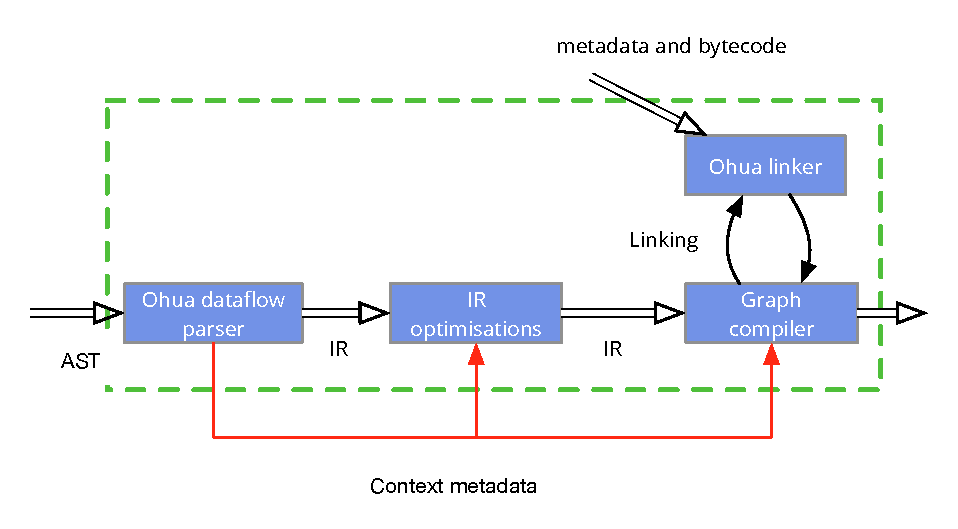
\includegraphics[width=\linewidth]{ohua-compiler-flow-with-ctx}
  \caption{Context information in the Ohua compiler flow}
  \label{fig:ohua-compiler-flow-with-ctx}
\end{figure}

At this point the subgraphs enclosed by the context are even more easily visible.
When we traverse the AST and we encounter a context introducing function like smap, we mark the enclosed function such that when it is being traversed all nodes inside are annotated with a reference to the smap starting node.
This overwrites any previous marker.
What we end up with, as a result, is an IR, where every node has, in its metadata, a reference to its closest context starting node.
The context starting node then has a reference to its nearest outer context and thus we can rebuild the entire context stack for each node afterwards.
For this we use dynamic programming by populating a HashMap with the stacks for each node, reusing previously computed results.
This can be done safely because Clojure standard library data structures like \texttt{Vector} are immutable and therefore safe to reuse.
After this process is completed we obtain a Map from node ids to completely resolved context stacks which is handed to subsequent transformations.

\section{Unwinding nested context}

Contexts like \texttt{if} and \texttt{smap} can be arbitrarily nested and interleaved in a program.
The detection algorithm, as described above, is able to correctly identify stacks of contexts for each node of the graph.
Subsequently we would like to `undo' each layer of context around each fetch to guarantee the node is only executed once per program run, which allows us to batch it.
This `undoing' operation should be reasonably efficient and yet easy to understand.

My context unwinding algorithm, which combines the if and smap transformations to deal with arbitrary nesting, uses the properties of contexts as mentioned above.
It unwinds one context at a time, dispatching to the appropriate handler, see Figure~\ref{fig:yauhau-rewrite-flow}, starting with the deepest nesting level.
The reason this results in a correct unwinding is that if a particular context has been unwound around a particular fetch, this fetch now lies in what was formerly the parent context.
Since this parent context cannot have been as deeply nested as the now unwound child context, it itself has not been unwound yet since we go from high nesting to low nesting.
At the same time since all contexts are eventually unwound the parent context has already been scheduled for unwinding.
By induction all contexts fetches are eventually unwound completely.

The correct order is achieved by using a work list of contexts to unwind.
The list is obtained by collecting the set of all context stacks on fetches, adding all substacks, ordering by length and finally mapping to the topmost element of the stack.
This last list is guaranteed to have no duplicates, due to the ``fully enclosed'' property of contexts.

In order to be as efficient as possible transformations are performed in a stateful way.
Individual transformation algorithms insert and delete nodes from the graph, insert and delete edges, as well as alter contexts for existing nodes or label new nodes with appropriate contexts.
Currently no sanity checks for the validity of those alterations are present, therefore the individual transformations themselves are responsible for preserving the integrity of the graph and its associated metadata structures.
This is not a hard limitation and might change in the future if we decide to allow more or user defined rewrites.

%
%\section{What is Context?}
%
%A context, as far as Ohua is concerned, is a programming construct which changes the behavior of subsequent sections of code.
%As an example the most basic context is the root context of an ohua \textt{algo} which changes the behavior of the functions within in so far as that they are executed once for each time the algo is executed.
%Another example is the \texttt{smap} context which casues functions within to be executet multiple times.
%Both of these contexts are control flow contexts which means they alter whether and how often functions are executed.
%Most contexts in ohua are represented as a pair of encapsulating operators which mark the beginning and end of the context respectively and the context itself influences the operators in between.
%The beginning marker sets up the altered behaviour and the end marker restores the original behavior.
%
%In case of the \texttt{algo} context the \texttt{algo-in} as start operator starts the execution and the \texttt{algo-out} operator as end operator collects the result.
%For \texttt{smap} the \texttt{smap} operator starts by executing the algorithm within once for each element in the structure being mapped and the \texttt{collect} operator restores the old behavior by waiting for as many elements as were in the mapped structure before returning them collectively to the next part of the program.
%
%\subsection{Arising problems}
%
%
%Control flow altering context such as smap or if pose a problem for yauhau.
%The idea behind our batching transformation is to find sets of pairiwise independent fetches and replacing them with a single, accumulated (batched) fetch.
%The accumulator would execute all fetches at once and return the results back into the appropriate place in the graph.
%However it is a simple operator and has to wait for all inputs before executing.
%This would pose an issue, were one of its inputs coming from the branch of a conditional, such as if.
%If the branch in question was not selected at runtime the input to the accumulator would be missing, preventing it from executing any of the fetches.
%Similarly with the map operation smap.
%Were one of the inputs to the accumulator originating from inside an smap the input could get several values instead of just one, a situation which the naive accumulator is unable to cope with.
%As a result we need to ensure all inputs to an accumulator are present at the same time and in the same quantity.
%In turn this means each of the pairwise parallel fetches has to be called the same number of times.
%The simplest way to do this is to remove all control flow context around a fetch operation, leaving it in the root context.
%Here we are guaranteed that any fetch will only ever be executed once.
%
%I should mention that there is an alternative strategy for handling this but it would require runtime scheduling.
%Scheduling offers more flexibility but at the same time also poses a substantially larger runtime overhead.
%Because of this we opted for a compile time rewrite approach.
%
%Haxl and muse both use runtime techniques to tackle this problem.
%In the case of Haxl it leverages the Haskell runtime (scheduler) whereas muse relies on a runtime AST and traversals on this AST.
%
%\subsection{Detection}
%
%In order to allow transformations as described in the following chapters which act upon and change context in the graph we must first find the contexts within the graph.
%In essence we would like to be able to reliably identify the subgraphs for each enclosing context in the graph.
%
%A simple solution would be to filter the graph for pairs of context begin and end operator and construct the set of nodes which satisfy the following conditions:
%\begin{enumerate}
%    \item The node is reachable from the begin operator
%    \item The end operator is reachable from the node
%\end{enumerate}
%The second condition is strictly not necessary since values cannot escape a surrounding context aside from through the and operator.
%Or more practically speaking if a value would escape a surrounding context without passing through the end operator the resulting program would be invalid and not executable.
%
%This is not only very inefficient\footnote{The inefficiency stems from the fact that this approch requires a partial graph traversal for each context.} but it is also difficult to assure that contexts are detected in the right order.
%
%In order to efficiently find the correct context layout I decided to use an algorithm which labels each node in the graph with its context.
%This can be achieved with a single, partially overlapping traversal of the graph.
%The basic algorithm is a breadth first traversal\footnote{A depth first traveral should yield the same result.} through the nodes of the graph and in the direction of the edges.
%Each step of the algorithm we cosider two nodes.
%An arbitrary current node and the parent node from which it was reached.
%During each step one of the following cases may occur
%\begin{enumerate}
%    \item \textbf{The current node was not visited previosly and does not open a new context.} Label the node with the context of the parent, add it to the visited nodes and enqueue it.
%    \item \textbf{The current node was not visited previously and opens a new context.} Label the node with the context of the parent plus a new context stack frame for the newly opened context. Add it to the visited nodes and enqueue it.
%    \item \textbf{The current node was not visited previously and closes a new context.} If the context matches the topmost context stack frame (is the closing operator), label it with the parents context stack with the topmost frame popped off and enqueue it.
%    \item \textbf{The current node was previously visited and assigned a context stack \textit{shorter} than the one of the parent.} Proceed as if the node had not been visited yet.
%    \item \textbf{The current node was previously visited and assigned a context stack \textit{longer or qual} to the one of the parent.} Ignore the node.
%\end{enumerate}
%
%The last case in particular hinges on the fact that contexts are always completely surrounded by their parent context.
%Or more formally if there is a context $c_0$ inside of which context $c_1$ is opened then all nodes inside $c_1$ are also in $c_0$.
%Therfore if node $n$ is reached with a context stack $s_1$ and was previously reached and labeled with the context stack $s_0$ and $|s_0| > |s_1|$ then $s_1 = s_0 + s_1' $ where $ |s_1'| > 0$.
